{
{\sffamily I det følgende, kaster vi et blik på detjlerne i programmets
billedbehandlingsmetoder. Efter en teknisk introduktion til digitale
billeder vises det, hvilke datastrukturer og metoder \emph{OpenCV}
stiller til rådighed, samt hvordan disse bruges, til at udtrække
regioner i digitale billeder. Endeligt vil vi undersøge, hvilke
svagheder vores implementation, til udtrækning af regioner, har.
}

\subsection{Digitale billeder}
I afsnit \ref{section_kort_intro} blev der givet en kort introduktion
til den digitale repræsentation af billeder. Det blev antaget, at en
pixel kunne antage værdier i mængden $\{0, 1\}$, men i praksis, kan
pixels godt antage andre værdier. Vi arbejder med billeder, hvor værdien
for hver pixel er repræsenteret ved tre 8 bit størrelser, hver med
værdier i mængden $\{0, 1, 2, \cdots, 254, 255\}$. Sammensætningen af de
tre værdier, som beskrives som kanaler eller farvebånd, kaldes for en
RGB-farve, hvor tallene repræsenteret ved $(R,G,B)$ angiver mængden af
hhv. rød, grøn og blå farve i en pixel. Et sådant billede, kaldes for et
RGB-billede. Vores korpus består af sådanne RGB-billeder med 8 bits, og
vi benytter derfor også denne repræsentation internt. Der er enkelte
undtagelser, hvor der kun bruges én kanal, således at vi arbejder med
gråtonebilleder. For en uddybning af billeders repræsentation henvises
til \cite{SIOlsen}.

Vi har også tidligere, i ligning \ref{billede_matrix},  vist, at et
digitalt billede kan skrives som en matrix. Ved denne matrix, kan man få
værdien for en pixel med koordinater $(x,y)$ ved elementet
$\mathbf{I}_{xy}$. Vi har altså, at x-aksen går fra øverste venstre
hjørne i nedadgående retning og y-aksen fra øverste venstre hjørne mod
højre. \emph{OpenCV} bruger dog et andet koordinatsystem, hvor akserne
er vendt om, som vist i figur \ref{opencv_koordinatsystem}. Man skal
derfor huske på at matricen, som\emph{OpenCV} bruger, er transponeret,
og vi skal derfor bytte om på koordinaterne. For at få værdien på den
pixel med koordinaterne $(x,y)$, skal vi altså bruge værdien
$\mathbf{I}_{yx}$, hvor de omvendte koordinater bør bemærkes.

\begin{figure}[!b]
    \centering
    \begin{picture}(122,55)
        \put(61, 50){$x$}
        \put(-10, 22){$y$}
        \put(0, 45){\circle*{3}}
        \put(-1, 45){\vector(1, 0){120}}
        \put(0, 45){\vector(0, -1){48}}

    \end{picture}
    \caption[]{Koordinatsystemet, som bliver brugt i \emph{OpenCV}.}
    \label{opencv_koordinatsystem}
\end{figure}

Billedematricen $\mathbf{I}$, repræsenteres i \emph{OpenCV} som et
dobbelt-array. I figur \ref{opencv_billedematrix} er vist hvordan
denne struktur ser ud, når vi har indlæst billedet givet i figur
\ref{billede_pixels}. Hvis billedet er indlæst i variablen \texttt{I},
kan vi i Python, tilgå pixelen med koordinater $(x,y) = (0,2)$ ved
$\textbf{I}_{2,0} =~$\texttt{I[2][0]}.

\begin{figure}[t]
    \begin{verbatim}
                        I = [ [0, 1, 0],
                              [1, 1, 1],
                              [0, 1, 0] ]
    \end{verbatim}
\vspace{-2em}
\caption{Repræsentation af billedematricen fra ligning
\ref{billede_pixels} i \emph{OpenCV}.}
\label{opencv_billedematrix}
\end{figure}

\subsection{Resultaters struktur\label{resultat_struktur}}
Indledningsvist vil vi introducere to vigtige datastrukturer, som vi
bruger fra \emph{OpenCV}. Alle datastrukturer og metoder fra
\emph{OpenCV}, har præfikset ``cv'', hvilket gør det let, at skelne
vores egne metoder fra dem der er givet i \emph{OpenCV}. Vi præsenterer
desuden en notation for datastrukturer, der er underlagt strukturen vist
i \eqref{types_class}.
\begin{multline}
    \textbf{class~} [\textit{name}] = \{ \\
    \shoveleft{\qquad[\textit{type}] : [\textit{varName}]} \\
    \shoveleft{\}}\shoveright{}
    \label{types_class}
\end{multline}
I \eqref{example_class} ses et eksempel på en struktur kaldet
\textbf{ExampleClass}.
\begin{multline}
    \textbf{class~} \textrm{ExampleClass} = \{ \\
    \shoveleft{\qquad\textbf{int} : \textit{intValue}} \\
    \shoveleft{\qquad\textbf{string} : \textit{stringValue}} \\
    \shoveleft{\qquad\textbf{int[2]} : \textit{arrayValues}} \\
    \shoveleft{\}}\shoveright{}
    \label{example_class}
\end{multline}
Bemærk, at en strukturs navn bliver skrevet med fed skrift i
brødteksten, når der refereres til en sådan. Ligeledes vil en strukturs
navn blive skrevet med fed i pseudokoden, hvis der refereres til den. Vi
kan definere en ny struktur, \textbf{NewClass}, som illustrerer dette, i
\eqref{new_class} herunder.
\begin{multline}
    \textbf{class~} \textrm{NewClass} = \{ \\
    \shoveleft{\qquad\textbf{ExampleClass} : \textit{exampleInstance}} \\
    \shoveleft{\qquad\textbf{string} : \textit{stringValue}} \\
    \shoveleft{\}}\shoveright{}
    \label{new_class}
\end{multline}
Med ovenstående notation kan vi nu beskrive to vigtige strukturer fra
\emph{OpenCV} kaldet \textbf{cvRect} og \textbf{cvConnectedComp}.

\subsubsection{cvRect}
Denne struktur beskriver et rektangel, ved at angive dets øverste venstre
hjørne og dets dimensioner. Strukturen vises i \eqref{cvRect_class}.
\begin{multline}
    \textbf{class~} \textrm{cvRect} = \{ \\
    \shoveleft{\qquad\textbf{int} : \textit{x}} \\
    \shoveleft{\qquad\textbf{int} : \textit{y}} \\
    \shoveleft{\qquad\textbf{int} : \textit{height}} \\
    \shoveleft{\qquad\textbf{int} : \textit{width}} \\
    \shoveleft{\}}\shoveright{}
    \label{cvRect_class}
\end{multline}
I vores implementation bruges denne struktur til at angive en regions
begrænsende rektangel. Vi vil i afsnit \ref{section_vurdering_regioner},
se, hvordan strukturen \textbf{cvRect} bruges i vurderingen af regioner.

\subsubsection{cvConnectedComp}
\emph{OpenCV} har en implementation af floodfill-metoden beskrevet i
afsnit \ref{subsec_floodfill}, som gør brug af en datastruktur kaldet
\textbf{cvConnectedComp}. Denne struktur bruges, til at beskrive den
region i billedet, som metoden fylder ud.  Strukturen er vist i
\eqref{cvConnectedComp_class}.
\begin{multline}
    \textbf{class~} \textrm{cvConnectedComp} = \{ \\
    \shoveleft{\qquad\textbf{double} : \textit{area}} \\
    \shoveleft{\qquad\textbf{float} : \textit{value}} \\
    \shoveleft{\qquad\textbf{cvRect} : \textit{rect}} \\
    \shoveleft{\}}\shoveright{}
    \label{cvConnectedComp_class}
\end{multline}
Strukturen indeholder en regions begrænsende rektangel og regionens
areal.

\subsubsection{Resultater}
Nu introduceres en ny struktur, som repræsenterer Pythons
\emph{dictionary}, forkortet \emph{dict}.  En \emph{dict} viser vi som i
\ref{def_dict}.
\begin{eqnarray}
    \langle[\textit{dictName}]\rangle = \{ [\textit{key}] : [\textit{data}] \}
    \label{def_dict}
\end{eqnarray}
Som et simpelt eksempel, kan vi konstruere en \emph{dict}
$\angles{LuckyNumbers}$, som indeholder personers lykketal:
% TeX-Gods, please forgive me :(
\begin{multline}
    \angles{LuckyNumbers} = \{ \qquad \textrm{Tom Cruise} : 4 , \\
    \textrm{Arthur Dent} : 42 \qquad\qquad\\
    \shoveleft{\}}\shoveright{}
    \label{lucky_dict}
\end{multline}
% In honor of the danish Tom Cruise
Data i en \emph{dict}, kan godt være af mere komplicerede typer, f.eks.
kan man have en anden \emph{dict}. Man kan således lave en hierakisk
struktur, som egner sig opbevaring af fundne regioner i et billede. Vi
ønsker at have hierakiet illustreret ved grammatikken i
\eqref{resultat_hieraki}.

\begin{equation}
    \begin{split}
        \textit{ImageRegions}  & \to  (\textit{RatioRegions~ImageRegions}')\\
        \textit{ImageRegions}' & \to  \textit{RatioRegions~ImageRegions}'\\
        \textit{ImageRegions}' & \to  \\
        \textit{RatioRegions}  & \to  (\textit{CutRegions~CutRegions~RatioRegions}')\\
        \textit{RatioRegions}' & \to  \textit{CutRegions~CutRegions}\\
        \textit{RatioRegions}' & \to  \\
        \textit{CutRegions}    & \to  (\textbf{CV\_RGB}, \textbf{cvConnectedComp})\textit{~CutRegions} \\
        \textit{CutRegions}    & \to
    \end{split}
    \label{resultat_hieraki}
\end{equation}

Vi har da, at et billede kan have et endeligt antal snitratioer, som man
ønsker at undersøge. Disse snitratioer, har enten to eller fire snit,
hvor der i hvert snit, er et antal fundne regioner, med en tilhørende farve.

Hver region i et snit bliver tildelt et \emph{id}, som er en
strengrepræsentation af regionens farve.  Hvis det antages, at regionens
farve er hvid, vil den have RGB-værdien $(255, 255, 255)$ og den får
derfor tildelt $id = \textrm{'255255255'}$. Vi konstruerer nu
$\angles{CutRegions}$, som indeholder de fundne regioner for et snit.
$\angles{CutRegions}$ er vist herunder i \eqref{CutRegions_dict}.
\begin{multline}
    \angles{CutRegions} = \{ \textit{~RegionId} : \\
    (\textbf{CV\_RGB~}\textit{color}, \textbf{cvConnectedComp~}\textit{region}) \}\quad
    \label{CutRegions_dict}
\end{multline}

\noindent I $\angles{CutRegions}$ bruges regionens id som nøgle. Vi kan nu
konstruere den \emph{dict} i niveauet over som vi betegner
$\angles{RatioRegions}$. Den ses i \eqref{RatioRegions_dict}.
\begin{eqnarray}
    \angles{RatioRegions} = \{ \textit{~CutNo} : \angles{CutRegions} \}
    \label{RatioRegions_dict}
\end{eqnarray}

\noindent $\angles{RatioRegions}$ holder alle regioner for en givet
snitratio.  Hvert snit, tilknyttet en snitratio, blev i afsnit
\ref{section_opdeling}, tildelt et id i mængden $\{0,1,2,3\}$. Vi bruger
snittets id som nøgle.  Data i $\angles{RatioRegions}$ er den instans af
$\angles{CutRegions}$ som tilhører snittet.

Det sidste niveau i hierakiet fra figur \ref{resultat_hieraki}, er endnu
en \emph{dict} givet ved $\angles{ImageRegions}$ vist i
\eqref{ImageRegions_dict}.
\begin{eqnarray}
    \angles{ImageRegions} = \{ \textit{~CutRatio} : \angles{RatioRegions} \}
    \label{ImageRegions_dict}
\end{eqnarray}

\noindent $\angles{ImageRegions}$ har nøglen $CutRatio$, som angiver en
snitratio til et billede. Hver snitratio har et antal snit, som endeligt
har et antal fundne regioner. Vi har således fået beskrevet den
struktur, som resultater bliver repræsenteret ved.

Resultatet fra en analyse på et billede, med snitratioerne $0.5$ og
$0.618$, ligner da det nedenstående:
%% !!! Bwadr-tex !!!
\begin{multline}
    \angles{ImageRegions} = \{ 0.5 : \{ 0 : \{ \textrm{'012345678'} : (color, region) \},\\
                                            \{ \textrm{'123456789'} : (color, region) \}
                                            \},\\
                                            \{ 1 : \{ \textrm{'012345678'} : ( \cdots ) \}, 
                                            \{ \cdots \} \}, \\
                              0.618 : \{ 0 : \{ \cdots \} \}, \{ 1 :
                              \cdots \}, \{ 2 : \cdots \}, \{ 3 : \cdots
                              \} \\
    \shoveleft{\}}\shoveright{}
    \label{CutRegions_dict}
\end{multline}

\subsection{Udtrækning af regioner}
I figur \ref{graphic_pipeline} er givet den række af manipulationer et billede
skal igennem i programmet, for at trække regioner ud af billedet, i
forhold til et givet snit. Resten af dette afsnit, vil omhandle den
egentlige implementation af denne fremgangmåde og problemerne
tilknyttet.  Indledningsvist vises, hvordan snit i billedet
repræsenteres.
\begin{figure}[!h]
    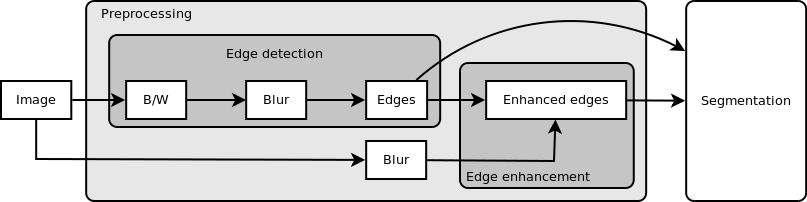
\includegraphics[width=\textwidth]{afsnit/implementation/billeder/billedbehandling/pipeline.png}
    \caption{Skema over grafiske modifikationer i forbindelse med
    udtrækning af regioner.}
    \label{graphic_pipeline}
\end{figure}

\subsubsection{Repræsentation af snit i billedet}
Metoderne i dette afsnit er ikke
specifikke for snitratioen $\varPhi$, men kan overføres til ethvert
andet snit i billedet, med en arbitrær snitratio.

Snit i et billede bliver repræsenteret ved et linjestykke. Vi
præsenterer nu datastrukturen \textbf{Line}, som består af et
linjestykkes to endepunkter.
\begin{multline}
    \textbf{class~} \textrm{Line} = \{ \\
    \shoveleft{\qquad\textbf{cvPoint} : \textit{p1}} \\
    \shoveleft{\qquad\textbf{cvPoint} : \textit{p2}} \\
    \shoveleft{\}}\shoveright{}
    \label{Line_class}
\end{multline}

\subsubsection{Præparation af billedet}
Det første skridt i præparation af billedet, er at detektere kanterne på
objekter i billedet.  Kanter detekteres i et sort/hvid-billede, så vi
starter med at lave en sort/hvid kopi af det originale billede. Inden
den egentlige kantdetektion, sløres det sort/hvide billede, således at
vi kun betragter kanter, som fremstår tydeligt i billedet.

I andet skridt af fremgangsmåden sløres det originale billede. Både i
sløringingen inden kantdetektion og denne bruges simpel sløring, som er
hurtigt og effektiv.

Sidste skridt er fremhævelse af de detekterede kanter. Det gøres ved at
oprette et nyt billede, med samme størrelse som originalbilledet. Alle
pixels, i det nye billede, farves sort. Dernæst kopieres alle pixels fra
det originale billede, over i det sorte billede, med undtagelse af de
pixels, hvor der er detekteret en kant. Derved forbliver kanterne sorte.
At lade kanterne være sorte kan have nogle utilsigtede konsekvenser. Vi
henviser til afsnit \ref{subsec_svagheder} for en gennemgang af disse.

Præparation af et billede er fremstillet som pseudokode i kodeboks
\ref{pseudo_prepare}.

\begin{lstlisting}[caption={Pseudokode for metoder til præparation af
    billeder.},captionpos=b,label={pseudo_prepare},numbers=left,
    frame=tb, breaklines=false, float=h]
def GetEdges(original, threshold1, threshold2):
    # Create images
    gray = cvCreateImage(cv.cvGetSize(original), 8, 1)
    out  = cvCreateImage(cv.cvGetSize(original), 8, 1)

    # Convert to B/W
    cvCvtColor(original, gray, CV_BGR2GRAY)

    # Simple blur
    cvSmooth(gray, out, CV_BLUR, 3, 3, 0)

    # Edge detect
    cvCanny(gray, out, threshold1, threshold2)

    return out

def EnhanceEdges(img, edges):
    workImage = cvCreateImage(cv.cvGetSize(original), 8, 3)

    # Superimpose the edges onto the image
    cvNot(edgeImage, edgeImage)
    cvCopy(img, workImage, edges)

    # Get the edges back to white
    cvNot(edges, edges)

    return workImage

def Preprocessing(original, thresholds):
    # Find edges
    edgeImage = GetEdges(original, threshold1, threshold2)

    # Blur
    blurImage = cvCreateImage(cv.cvGetSize(original), 8, 3)
    cvSmooth(original, blurImage, CV_BLUR, 3, 3, 0)

    # Enhance edges
    enhanced = EnhanceEdges(blurImage, edges)

    return (enhanced, edges)

\end{lstlisting}

\subsubsection{Segmentering med floodfill-metoden}
% Plan
% Vi optimerer, maler ikke alle pixel
% Vi bruger det kantdetekterede billede
% Vi laver linjestykker
% Vi bemærker at ikke hele regionen bliver fyldt ud
% Vi maler to gange, men det er en fejl
% Vi retter koden
Vi beskriver nu metoden, til at trække regioner ud af et præpareret
billede. Metoden bygger videre på beskrivelsen givet i
\ref{sammensaetning_af_metoder}, hvor floodfill-metoden bruges på hver
pixel langs et snit. I praksis er denne fremgangsmåde meget langsom,
især med store billeder. Vi vil derfor komme frem til en metode, som kun
bruger floodfill-metoden på de nødvendige pixels.

Vi bruger de detekterede kanter, til at hjælpe med at segmentere
billedet, da vi vil bruge floodfill med en ny farve når vi passerer en
kant. Vi trækker derfor de punkter ud, hvor en kant krydser snittet, ved
metoden vist i kodeboks \ref{pseudo_GetPoints}.

\begin{lstlisting}[caption={Pseudokode for metode til at finde punkter,
    hvor en kant krydser snittet.},captionpos=b,label={pseudo_GetPoints},numbers=left,
    frame=tb, breaklines=false, float=h]
def GetPoints(edges, cut):
    points = []
    for pixel on cut:
        if not (color(pixel) == 0):
            points += pixel
\end{lstlisting}

Vi repræsenterer snittet som et linjestykke og vi kan således dele dette
i mindre segmenter mellem kanter. Et eksempel på et horisontalt snit er
vist i figur \ref{impUdtraek_kantpunkter}.

\begin{figure}[!h]
    \centering
    \begin{picture}(240,30)
        \put(0, 10){$A$}
        \put(3, -5){\line(0, 1){10}}

        \put(82, 10){$e_1$}
        \put(85, 0){\circle*{3}}

        \put(102, 10){$e_2$}
        \put(105, 0){\circle*{3}}

        \put(134, 10){$e_3$}
        \put(137, 0){\circle*{3}}

        \put(158, 10){$e_4$}
        \put(161, 0){\circle*{3}}

        \put(200, 10){$e_5$}
        \put(203, 0){\circle*{3}}

        \put(221, 10){$e_6$}
        \put(224, 0){\circle*{3}}

        \put(233, 10){$B$}
        \put(236, -5){\line(0, 1){10}}

        \put(3, 0){\line(1, 0){233}}
    \end{picture}
    \caption[]{Punkter, hvor der er en kant der krydser snittet.}
    \label{impUdtraek_kantpunkter}
\end{figure}

Vi vil nu bruge floodfill således, at hvert linjestykke bliver tildelt
en tilfældig farve, som endnu ikke er blevet givet til et andet
linjestykke, og maler hvert linjestykke med denne. Naivt ville man bruge
floodfill på midten af hvert linjestykke, men dette er ikke holdbart, da
vi ikke kan være sikre på, at hele linjestykket farves. Figur
\ref{floodfill_taerskel_problem} viser, at det ikke er
ligemeget \emph{hvor} på linjestykket man bruger floodfill, når vi har
med arbitrære billeder at gøre. Vi vil derfor gå langs snittet og bruge
floodfill på alle pixels, som endnu ikke er blevet farvet af floodfill.
Hver gang vi bruger floodfill, returneres en instans af strukturen
\textbf{cvConnectedComp}.

Vi skal også være sikre på, at floodfill returnerer hele den fundne
region. Den returnerede \textbf{cvConnectedComp} er den \emph{senest
farvede} region. I figur \ref{floodfill_return_entire_region} vises en
situation, hvor vi ikke har farvet hele linjestykket, og når vi udvider
den fundne region, returnerer floodfill kun et undersæt af alle pixels i
regionen. Vi skal derfor bruge floodfill mere end én gang, for at sikre
os, at hele regionen returneres. Vi har dertil udviklet pseudokoden i
kodeboks \ref{pseudo_udtraek_org}.

\begin{figure}[h]
    \setlength\fboxsep{0pt}
    \setlength\fboxrule{0.5pt}
    \centering
    \fbox{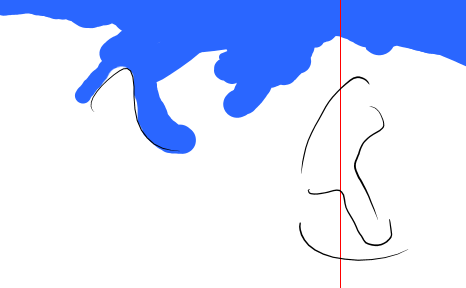
\includegraphics[width=0.8\textwidth]{afsnit/implementation/billeder/billedbehandling/floodfill_color.png}}
    \caption[]{Problemet med floodfill-metoden i billeder med flere
    farver. Hvid farve er ikke blevet malet af floodfill-metoden endnu.
    Den lyseblå region dækker ikke hele linjestykket ned til kanten.}
    \label{floodfill_taerskel_problem}
\end{figure}

\begin{lstlisting}[caption={Original pseudokode til udtrækning af
    regioner. Denne kan returnere den samme region flere
    gange.},captionpos=b,label={pseudo_udtraek_org},numbers=left,
    frame=tb, breaklines=false, float=h]
for lineSegment in Cut:
    # Get a new color that is not in the component dictionary
    color = getRandomColor()
    region = cvConnectedComp()

    for pixel in lineSegment:

        # Check if the color of the pixel equals current color
        if not (color(pixel) ==  color):

            # Check if the color of the pixel are in the saved regions
            if not (color(pixel) in CutRegions):
                cv.cvFloodFill(img, pixel, color, lowerThres, upperThres, region)

    # Color the last pixel again to make sure that
    # the returned component is the entire region
    cv.cvFloodFill(img, pixel, color, lowerThres, upperThres, region)

    # Put the results in the CutRegions-dictionary
    CutRegions[color.toString()] = (color, region)
\end{lstlisting}

\begin{figure}[p]
    \setlength\fboxsep{0pt}
    \setlength\fboxrule{0.5pt}
    \centering
    \subfloat[En tilføjelse til den lyseblå region. Det begrænsende
    rektangel svarer kun til udvidelsen.]{
        \label{new_reg_small_box}
        \fbox{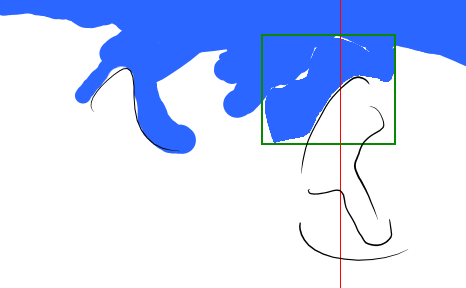
\includegraphics[angle=0,width=0.8\textwidth]{afsnit/implementation/billeder/billedbehandling/floodfill_color_new_reg_small_box}}
        }\\
    \subfloat[Ved at bruge floodfill på regionen igen, markeres hele den
    lyseblå region, som vi ønsker.]{
        \label{new_reg_big_box}
        \fbox{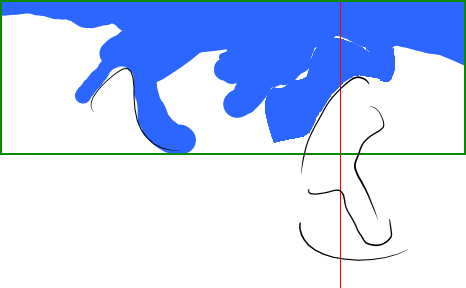
\includegraphics[angle=0,width=0.8\textwidth]{afsnit/implementation/billeder/billedbehandling/floodfill_color_new_reg_big_box}}
        }
    \caption[]{
    Floodfills opførsel ved udvidelse af regioner.
    }
    \label{floodfill_return_entire_region}
\end{figure}

Vi har i kodeboks \ref{pseudo_udtraek_org}, forsøgt at tage højde for
problemet nævnt i figur \ref{new_reg_small_box}, ved et ekstra kald til
\texttt{cvFloodFill} i linje 17, som vil farve den sidste pixel en
ekstra gang, for at sikre at hele regionen returneres. Kaldet gør dog
også, at der \emph{altid} bliver returneret en region for hvert segment.
Dette er ikke ønskværdigt, specielt ikke hvis vi er sprunget over alle
pixels på et linjestykke. Dette sker, netop når hele regionen allerede
er blevet fyldt ud. I praksis betyder dette, at der kan blive fundet
flere regioner i et billede end der reelt er. I bilag \ref{appendix_bug}
er givet en håndkørsel af den fejlende kode.

Fejlen i linje 17 har eksisteret selv under vores kørte eksperiment i
afsnit \ref{section_naiv_koersel}.  Vi har fjernet duplikaterne på
databaseniveau, men metoden er senere blevet rettet til at have den
korrekte opførsel. Den reviderede metode er vist i kodeboks
\ref{pseudo_udtraek_rev}.

\begin{lstlisting}[caption={Revideret pseudokode til udtrækning af
    regioner. Returnerer ingen
    duplikater.},captionpos=b,label={pseudo_udtraek_rev},numbers=left,
    frame=tb, breaklines=false, float=h]
for lineSegment in Cut:
    # Get a new color that is not in the component dictionary
    color = getRandomColor()

    # Set region to None, as we have not yet found any
    region = None

    for pixel in lineSegment:

        # Check if the color of the pixel equals current color
        if not (color(pixel) ==  color):

            # Check if the color of the pixel are in the saved regions
            if not (color(pixel) in CutRegions):
                # Now we've got a new region
                region = cvConnectedComp()
                cv.cvFloodFill(img, pixel, color, lowerThres, upperThres, region)

                # Color the pixel again to make sure that
                # the returned component is the entire region
                cv.cvFloodFill(img, pixel, color, lowerThres, upperThres, region)

    # If we have found a region, then put the result in the CutRegions-dictionary
    if not (region is None):
        CutRegions[color.toString()] = (color, region)
\end{lstlisting}

Metoden i kodeboks \ref{pseudo_udtraek_rev} bruger \texttt{cvFloodFill}
to gange, hver gang man møder en ikke-farvet pixel. Dette koster lidt
køretid, men sikrer, at man altid får hele regionen returneret i
\textbf{cvConnectedComp}.

%Man kan fristes til at flytte kaldet i linje
%21 ind i \texttt{if}-sætningen i linje 24, men dette åbner op for
%svagheden igen, da vi ikke ved, om den sidste pixel tilhører den
%aktuelle region. Derfor er vi nødt til at ofre lidt køretid, for at
%være sikre på resultatet. Metoden benytter et ``først til
%mølle''-princip, hvor en pixel, når den først et blevet tilknyttet en
%region, altid vil tilhøre denne.

Vi trækker dog kun de regioner ud som rører \emph{snittet}. I kapitel
\ref{chap_detektion} indførtes et margin, således at også regioner, som
ligger tæt på snittet, kan trækkes ud. Vi vil nu udvide pseudokoden i
kodeboks \ref{pseudo_udtraek_rev} til også at trække regioner ud, som
krydser margin. Vi navngiver metoden \texttt{GetCutRegions}, og den
tager et snit som argument. Metoden ses i kodeboks
\ref{pseudo_udtraek_margin}. Metoden trækker først regioner ud med
hensyn til det nedre margin, så med hensyn til det øvre margin og til
sidst med hensyn til selve snittet. Alle regioner gemmes i den samme
instans af $\angles{CutRatios}$. For selve udregningen af margin,
henvises til afsnit \ref{subsec_margin_udregning}.

\begin{lstlisting}[caption={Pseudokode til udtrækning af regioner med
    margin.},captionpos=b,label={pseudo_udtraek_margin},numbers=left,
    frame=tb, breaklines=false, float=h]
def GetCutRegions(img, edges, cut):
    # Calculate lowerMargin and upperMargin
    (lowerMargin, upperMargin) = calculateMargins(cut)
    Cuts = [lowerMargin, upperMargin, cut]

    # Initialize an empty CutRegions-dict
    CutRegions = {}

    for Cut in Cuts:
        # Use the edge image to find the line segments
        for lineSegment in Cut:
            # Get a new color that is not in the component dictionary
            color = getRandomColor()

            # Set region to None, as we have not yet found any
            region = None

            for pixel in lineSegment:

                # Check if the color of the pixel equals current color
                if not (color(pixel) ==  color):

                    # Check if the color of the pixel are in the saved regions
                    if not (color(pixel) in CutRegions):
                        # Now we've got a new region
                        region = cvConnectedComp()
                        cv.cvFloodFill(img, pixel, color,
                                    lowerThres, upperThres, region)

                        # Color the pixel again to make sure that
                        # the returned component is the entire region
                        cv.cvFloodFill(img, pixel, color,
                                    lowerThres, upperThres, region)

            # If we have found a region,
            # then put the result in the CutRegions-dictionary
            if not (region is None):
                CutRegions[color.toString()] = (color, region)

    return CutRegions
\end{lstlisting}

Vi kan nu kombinere alle metoderne, således at vi kan trække regioner ud
af arbitrære billeder. Til dette bruges pseudokoden vist i kodeboks
\ref{pseudo_udtraek_all}.

\begin{lstlisting}[caption={Fuld udtrækning af regioner i et arbitært
    billede.},captionpos=b,label={pseudo_udtraek_all},numbers=left,
    frame=tb, breaklines=false, float=h]
def NaiveExtraction(original):
    # Preprocess the image
    (enhanced, edges) = Preprocessing(original, thresholds)

    # Get regions
    return GetCutRegions(enhanced, edges, cut)
\end{lstlisting}

\subsection{Svagheder\label{subsec_svagheder}}
Den endelige metode, for udtrækning af regioner, med hensyn til et givet
snit i billedet, har nogle svagheder. Den første er allerede nævnt:
Metoden trækker kun regioner ud \emph{med hensyn} til et snit. Dette
betyder, at kun regioner, som rører margin eller selve snittet, bliver
trukket ud. Foregående skal tages helt bogstaveligt, i den forstand, at
vi \emph{skal} have, at en region har en pixel enten på det nedre
margin, det øvre margin eller på selve snittet, for at blive trukket ud.
Vi kan altså godt have interessante regioner, som faktisk har mindst én
kant af sit begrænsende rektangel inden for margin, som ikke bliver
trukket ud. Et eksempel er vist i figur \ref{respect_to_cut}, hvor den
sorte region ikke vil blive trukket ud, selvom den har to kanter inden
for margin.

\begin{figure}[h]
    \setlength\fboxsep{0pt}
    \setlength\fboxrule{0.5pt}
    \centering
    \fbox{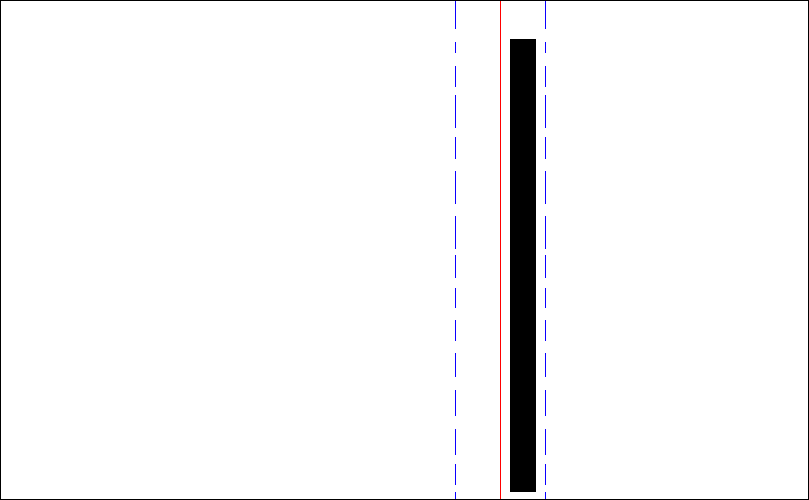
\includegraphics[width=0.8\textwidth]{afsnit/implementation/billeder/billedbehandling/respect_to_cut.png}}
    \caption[]{Sort region, som ikke bliver trukket ud af billedet.
    Selvom regionens begrænsende rektangel ligger inden for margin, så
    krydser regionen hverken nedre margin, øvre margin eller selve
    snittet. Derfor opdages regionen ikke.}
    \label{respect_to_cut}
\end{figure}

\subsubsection{Valg af tilfældige RGB-værdier}
Man skal endvidere være opmærksom på, at hver gang vi markerer en ny
region, tildeles denne en tilfældig farve.  Vi kan, i vores valg af
farve, være uheldig og vælge en, som bliver brugt i det originale
billede. Når vi kalder \texttt{cvFloodFill} igen, for at være sikre, at
hele regionen bliver returneret, kan vi smelte to regioner sammen, som
egentlig ikke burde hænge sammen. I figur \ref{floodfill_colors} er
denne situation vist på det præparerede billede fra figur \ref{bathers}.
Ligeledes kan vi være uheldige, at støde på en pixel, som har en farve
lig med en allerede farvet region. I dette tilfælde, vil denne pixel
blive anset som værende del af en eksisterende region, hvilket
resulterer i at vi ikke bruger \texttt{cvFloodFill} på denne. Vi kan dog
håbe, at denne pixel bliver inkluderet i den efterfølgende iteration.
Vi vælger aldrig, at farve en region med en farve, som allerede er brugt
til en anden region, men vi kan være uheldige og vælge en farve, som
ligger inden for floodfill-metodens tilladte afvigelse, således at to
regioner smeltes sammen.

\begin{figure}[h]
    \setlength\fboxsep{0pt}
    \setlength\fboxrule{0.5pt}
    \centering
    \subfloat[Originalt præpareret billede inden vi vælger en tilfældig
    farve til floodfill.]{
        \label{colors_1}
        \fbox{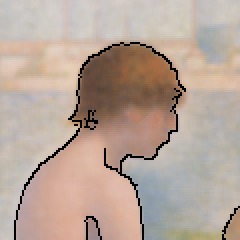
\includegraphics[width=0.3\textwidth]{afsnit/implementation/billeder/billedbehandling/pre_floodfill_1}}}\hspace{1em}
    \subfloat[Region fyldes med farve lig eksisterende pixels i
    billedet. Pixels i drengens hår har nu samme farve som kroppen.]{
        \label{colors_2}
        \fbox{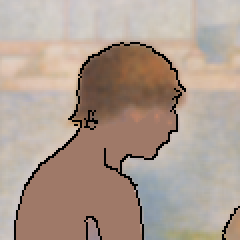
\includegraphics[width=0.3\textwidth]{afsnit/implementation/billeder/billedbehandling/pre_floodfill_2}}}\\
    \subfloat[Når floodfill bruges en ekstra gang, for at være sikker på
    at hele regionen returneres, smeltes drengens krop og hår sammen.]{
        \label{colors_3}
        \fbox{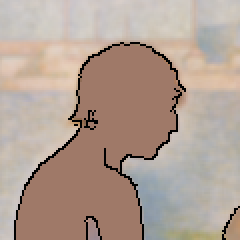
\includegraphics[width=0.3\textwidth]{afsnit/implementation/billeder/billedbehandling/pre_floodfill_3}}}\hspace{1em}
    \subfloat[Hvis den første region havde fået en anden farve, ville vi
    ikke have smeltet to regioner sammen.]{
        \label{colors_4}
        \fbox{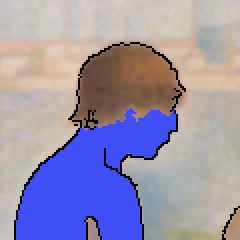
\includegraphics[width=0.3\textwidth]{afsnit/implementation/billeder/billedbehandling/pre_floodfill_4}}}\\
    \label{floodfill_colors}
    \caption[]{Uheldige valg af tilfældig farve til regioner.}
\end{figure}

\subsubsection{Ikke-sammenhængende regioner}
Metoden i kodeboks \ref{pseudo_udtraek_margin}, trækker højest én region
ud per segment. Dette giver mening, set i lyset af hvad
udtrækningsmetoden er blevet udviklet til, nemlig udtrækning af
\emph{sammenhængende regioner} afgrænset ved kantdetektion. I afsnit
\ref{section_computer_betragter} antog vi, at interessante regioner i et
billede, er tydeligt afgrænset. En region er ikke tydeligt afgrænset,
hvis vi faktisk \emph{har} flere regioner indenfor et segment. I figur
\ref{usammenhaengende_region} betragter vi en hypotetisk situation, hvor
en region ikke har været tydeligt afgrænset. Billedet i figur
\ref{usammenhaengende_region}, illustrerer et billede, som allerede er
blevet segmenteret ved metoden i kodeboks \ref{pseudo_udtraek_margin}.
De sorte cirkler markerer dér, hvor vi har fundet kanter, som krydser
snittet. Vi har altså fem segmenter på snittet. På det længste segment,
ser vi, at den mørkeblå region er blevet afbrudt af en tidligere fundet
region. Den mørkeblå region er således ikke sammenhængende. Metoden
returnerer kun den nederste mørkeblå region, da vi ikke kan forbinde
de to mørkeblå regioner. Vi mister derfor informationen om at der
faktisk befinder sig en region i midten af billedet.

Denne opførsel, er en konsekvens af vores antagelse, om at interessante
regioner er tydeligt afgrænset. Vi accepterer derfor, at situationen i
figur \ref{usammenhaengende_region} kan forekomme, og at vi derfor kan
undlade at trække enkelte regioner ud.

\begin{figure}[t]
    \setlength\fboxsep{0pt}
    \setlength\fboxrule{0.5pt}
    \centering
    \fbox{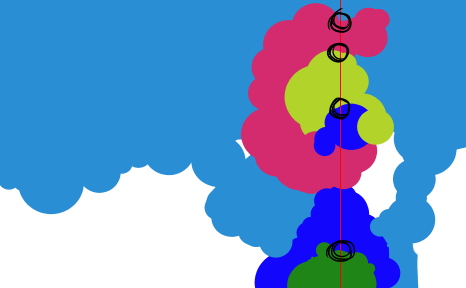
\includegraphics[width=0.8\textwidth]{afsnit/implementation/billeder/billedbehandling/usammenhaengende_region.png}}
    \caption[]{Et segmenteret billede. Sorte cirkler angiver steder,
    hvor vi har detekteret en kant, der krydser snittet. Den mørkeblå
    region er usammenhængende over snittet, da den afbrydes af den røde
    region. Kun den nederste mørkeblå region er blevet returneret.}
    \label{usammenhaengende_region}
\end{figure}

\subsubsection{Usikkerhed ved fremhævelse af kanter}
De fremhævede kanter, tegnes i det slørede billede med sort farve, som
vælges uanset hvilke farver, der er brugt i maleriet i forvejen. Vi kan
derfor støde på problemer med mørke malerier eller lokalt i mørke
områder af et billede. Vi kan også være uheldige, at komme til at
forbinde to regioner, ved at markere kanterne med sort.

På grund af, at kanterne fremhæves ved at male i billedet, kan vi, ved
floodfill-metoden, komme til at male kanter, som har samme retning, som
det snit vi betragter. Dvs, at lodrette kanter kan blive malet ved
vertikale snit og omvendt kan vandrette kanter risikere at blive malet
ved horisontale snit.

\subsection{Andre tilgange og forbedringer}
Dette afsnit vil kort nævne andre fremgangsmåder, vi har prøvet, for at
trække regioner ud af et billede. Vi har tidligt i udviklingen af
programmet, eksperimenteret både med Octave og Matlab. Til at starte
med, har vi brugt disse sprog til at komme problemstillingen nærmere,
og udvikle naive implementationer af enkelte algoritmer. Vi ser nu på
hvad der kan gøres for at forbedre udtrækningen af regioner.

\subsubsection{Udtrækning af alle regioner}
At vi kan have regioner som ikke trækkes ud af billedet, som i figur
\ref{respect_to_cut}, er beklagelig, men kan løses ved pseudokoden i
kodeboks \ref{pseudo_fix}.  Her er tanken, at man i stedet for kun at
trække regioner ud på margin og selve snittet, så gøres det på hver
pixel mellem margin. På denne måde kan regioner, som den i figur
\ref{respect_to_cut}, trækkes ud af billedet. Vores implementation gør
dog ikke dette. Når regioner kun trækkes ud, med hensyn til et snit, kan
vi ved denne metode heller ikke garantere en fuld segmentering af
billedet.

\begin{lstlisting}[caption={Pseudokode til udtrækning af regioner med
    margin.},captionpos=b,label={pseudo_fix},numbers=left,
    frame=tb, breaklines=false, float=h]
def FixGetRegions(img, edges, cut):
    # Calculate lowerMargin and upperMargin
    (lowerMargin, upperMargin) = calculateMargins(cut)

    for pixel in (lowerMargin to upperMargin):
        # Extract regions
        pass
\end{lstlisting}

Vi har også eksperimenteret med, først at skalere billedet ned, inden
man trak regioner ud. Dette gør nemlig, at kanterne forbliver intakte,
mens farverne, til en vis grad, bliver mere ensartede. Vi stødte dog på
problemer når billedet skulle skaleres op igen, eller rettere, få
resultaterne skalleret op, så de passede til originalbilledet. Vi mister
også meget præcision, når vi bruger et nedskaleret billede til at finde
regioner i.


I præparationen af billedet, vil vi gerne have, at farverne i billedet
bliver ensartede, men vi ønsker også at bibeholde kanterne. Vi forsøgte
at bruge en metode i \emph{OpenCV}, der hedder
\texttt{cvPyrMeanShiftFiltering}, som netop segmenterer billedet efter
hvilke farver der ligner hinanden, men en fejl i biblioteket forsagede
altid en segmenteringsfejl i det underliggende C-program. Vi blev siden
gjort opmærksom på en sløringsmetode af Perona og
Malik\cite{perona1990scale}, hvor det grafiske resultat tilnærmer sig
det ønskede. Kun i Octaves \emph{Image}-pakke er denne implementeret. Vi
lavede en hurtig afprøvning, hvor resultatet fra denne metode blev
analyseret, men på basis at det endelige resultat, vurderede vi, at vi
godt kunne nøjes med at fremhæve kanterne i billedet efter en simpel
sløring.

\subsubsection{Bedre fremhævelse af kanter}

\emph{OpenCV} gør det faktisk muligt, at bruge en maske, så man kan
kalde \texttt{cvFloodFill} med et kantdetekteret billede, således at man
ikke maler over de steder i billedet, hvor der er detekteret en kant. I
praksis viste det sig, at være yderst besværligt at bruge denne
funktion, da det kantdetekterede billede skal være to pixel større, i
hver dimension --- det kantdetekterede billede skal have en ramme, på én
pixel. En meget naiv løsning, hvor pixels kopieres én ad gangen, var
tidskrævende på store billeder og vi beholdt derfor de sorte kanter.
Alternativt kunne man beskære det originale billede, men vi besluttede,
at vi ikke ville manipulere med dimensionerne på vores inddata og bevare
det originale billede.

\subsubsection{Optimeringer}
Et hurtigt kig på arbejdsgangen i figur \ref{graphic_pipeline}, viser
allerede mindst ét sted, hvor vi kan optimere programmet. Billedet bliver
nemlig sløret to steder, både i forbindelse med kantdetektion og den
generelle sløring. Det er derfor oplagt, kun at sløre billedet én gang
og passere det slørede billede videre, som argument til de metoder, som
skal bruge det. Dette kan dog kun gøres, hvis vi ønsker at bruge den
samme sløringsmetode, til de to billeder.

Endvidere, kan selve udtrækningen af regioner måske forbedres, ved at bruge
sløring ved statistisk median. Denne metode har vi dog ikke fået testet
ordentlig igennem. Ved brug af en anden sløringsmetode, kunne det godt
tænkes, at fremhævelse af kanter bliver helt overflødig

}

% vim: set tw=72 spell spelllang=da:
